%%%%%%%%%%%%%%%%%%%%%%%%%%%%%%%%%%%%%%%%%%%%%%%%%%%%%%%%%%%%%%%%%%%%%%%%%%%%%%%
%% Copyright (c) 2010, 2022 Contributors to the Eclipse Foundation
%%
%% See the NOTICE file(s) distributed with this work for additional
%% information regarding copyright ownership.
%%
%% This program and the accompanying materials are made available under the terms
%% of the MIT License which is available at https://opensource.org/licenses/MIT
%%
%% SPDX-License-Identifier: MIT
%%%%%%%%%%%%%%%%%%%%%%%%%%%%%%%%%%%%%%%%%%%%%%%%%%%%%%%%%%%%%%%%%%%%%%%%%%%%%%%

% Package position
\newcommand{\pkgdocuposition}{
Figure~\ref{fig:pkg:position} shows the \textit{position} package.

\begin{figure}[H]
  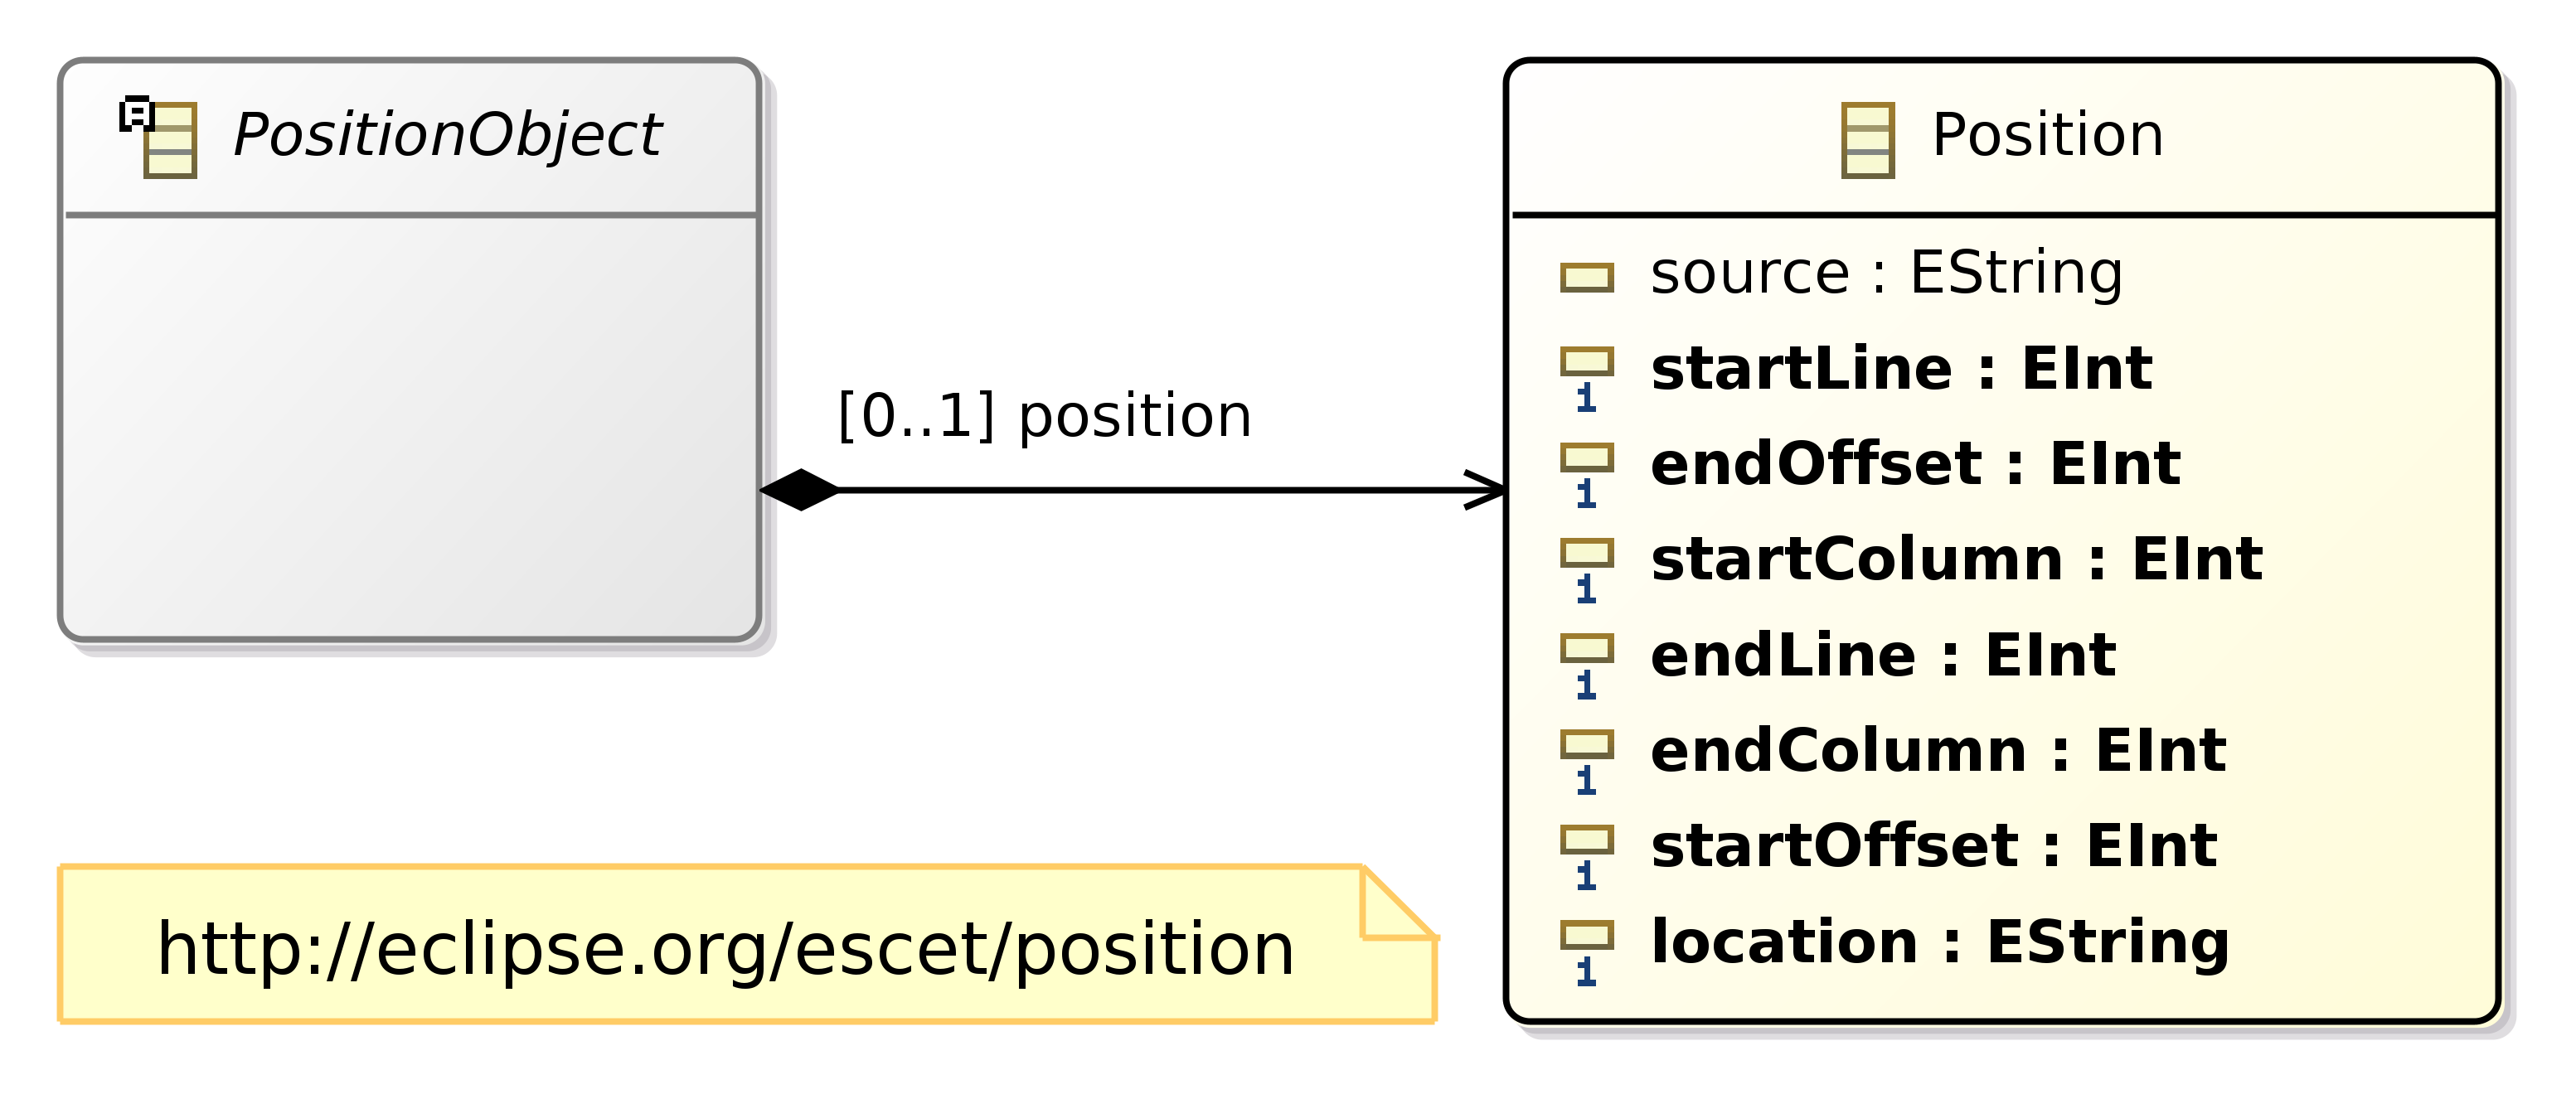
\includegraphics[width=\textwidth]{../model/position.png}
  \caption{\textit{position} package}\label{fig:pkg:position}
\end{figure}

The position package contains classes used to represent position information,
for source tracking. A position is represented as a continuous region in a
textual source (the \emph{source text}).

The \positionclass{Position} class represents actual position information.
The abstract \positionclass{PositionObject} class can be used as a base class
for other classes, and allows those classes to store position information.
}

% Position (class)
\newcommand{\clsdocuPosition}{
Position (source tracking) information.

\begin{constraints}
\citem{Position.lines}
  The \texttt{startLine} must be smaller than or equal to the \texttt{endLine}.
\citem{Position.columns}
  If the \texttt{startLine} is equal to the \texttt{endLine}, the
  \texttt{startColumn} must be smaller than or equal to the \texttt{endColumn}.
\citem{Position.offsets}
  The \texttt{startOffset} must be smaller than or equal to the
  \texttt{endOffset}.
\end{constraints}
}

\newcommand{\featdocuPositionendColumn}{
The 1-based column index of the end (inclusive) of the position region, with
respect to the start of the source text.

\begin{constraints}
\citem{Position.endColumnValue}
  Value must be greater than or equal to one.
\end{constraints}
}

\newcommand{\featdocuPositionendLine}{
The 1-based line index of the end (inclusive) of the position region, with
respect to the start of the source text.

\begin{constraints}
\citem{Position.endLineValue}
  Value must be greater than or equal to one.
\end{constraints}
}

\newcommand{\featdocuPositionendOffset}{
The 0-based byte index of the end (inclusive) of the position region, with
respect to the start of the source text.

\begin{constraints}
\citem{Position.endOffsetValue}
  Value must be greater than or equal to zero.
\end{constraints}
}

\newcommand{\featdocuPositionlocation}{
The location of the source file that contains the position. Must be an absolute
local file system path, with platform specific path separators. The path does
not have to refer to an existing file. That is, it may not be assumed that a
file with that path actually exists on disk.
}

\newcommand{\featdocuPositionsource}{
Optional source identification. Usually, this is a file name.
}

\newcommand{\featdocuPositionstartColumn}{
The 1-based column index of the start (inclusive) of the position region, with
respect to the start of the source text.

\begin{constraints}
\citem{Position.startColumnValue}
  Value must be greater than or equal to one.
\end{constraints}
}

\newcommand{\featdocuPositionstartLine}{
The 1-based line index of the start (inclusive) of the position region, with
respect to the start of the source text.

\begin{constraints}
\citem{Position.startLineValue}
  Value must be greater than or equal to one.
\end{constraints}
}

\newcommand{\featdocuPositionstartOffset}{
The 0-based byte index of the start (inclusive) of the position region,
with respect to the start of the source text.

\begin{constraints}
\citem{Position.startOffsetValue}
  Value must be greater than or equal to zero.
\end{constraints}
}

% PositionObject (abstract class)
\newcommand{\clsdocuPositionObject}{
Base class for other classes, facilitating the storage of position information.
}

\newcommand{\featdocuPositionObjectposition}{
Optional position information.
}
